\documentclass[11pt,a4paper]{IEEEtran}

% some very useful LaTeX packages include:

\usepackage{cite}
\usepackage{graphicx}
\usepackage{url}
\usepackage{amsmath}
\usepackage{subcaption}

\begin{document}
	\title{Stochastic Gradient Descent: Overview}
	\author{Adam Loch, Szymon Wojciechowski}
	\markboth{Optimization Methods: Theory - Report}{}
	\maketitle

\section{Introduction}
This paper is presenting a general description of Stochastic Gradient Descent algorithm and results of work done to implement it. Authors prepared application and set of example images that can help to understand the algorithm way of working.
\section{Stochastic Gradient Optimization}
\textbf{Stochastic Gradient Descent} (SGD) - is an modification of gradient descent optimization algorithm, widely used for optimization of neural networks \cite{Ruder16} or fitting regression models. The goal of algorithm is to minimize an multivariable function $J(\theta_0, \theta_1 ... \theta_n )$ for which denoted $\theta_n$ is an parameter of optimized model. Objective function must have a form:

$$ J(\Theta) = \frac{1}{k}\sum_{i=1}^{k} Q_i(\Theta) $$

where $Q_i$ can be associated with $i$-th observation in the dataset. The algorithm starts with randomly selected parameters $\theta$. In each iteration (step) algorithm is updating parameters in such way:

$$ \theta = \theta - \eta \cdot \nabla_\theta J( \theta) $$

where $\eta$ is a learning rate parameter of algorithm and $\nabla_\theta J(\theta)$ is gradient of the function. To understand that it can be said that algorithm is starting at some point on surface (generated by objective function) and in each iteration it is moving toward the direction where the descent is highest. It continues to do so until the satisfying minima is reached, or limit of iterations (calculation time) is reached.

The difference between stochastic gradient descent and generic (batch) gradient descent is that update in each iteration is calculated only on randomly selected subset of observations. It make a route to minima noisier than in full-calculations approach, but also it reduces amount of computations needed which makes it faster.

\subsection{Gradient computation}

It is essential to make gradient calculations for discussed algorithm. The general gradient formula can be defined as a vector of derivatives for each of the function variables $x_n$

$$ \nabla f = \left[\frac{\partial f}{\partial x_1}, \dots, \frac{\partial f}{\partial x_n}\right] $$

Unfortunatly, calculating derivatives in algorithm would require solving differential equation of whole formula, which in case of generic algorithm implementation is not trivial and sometimes impossible.

However it is possible to calculate numerical gradient using \textit{Central-Difference Formulas}\cite{Mathews:1998}. Assuming that $x \pm h$ is in neighbourhood of $x$, than

$$ f'(x) \approx \frac{f(x+h)-f(x-h)}{2h} $$

Such assumption simplyfy calculations but with a cost of truncation error: $O(h^2)$. It implies that all calculations are not precise, but as long as this value is small enough, algorithm will be sufficiently precise.

\section{Goals}
The goal is to prepare an application that will be able to present how algorithm is running optimization. It requires:
\begin{itemize}
\item Own implementation of SGD
\item Own implementation of numeric gradient
\item Visualization of steps performed by algorithm
\end{itemize}
To satisfy second requirements, it is needed that

\textit{Objective function must be a function of two variables}.

For programming authors selected Python language, which offers and efficient implementation of numerical computations \cite{oliphant_guide_2006}. It also provides a package for creating interactive plots \cite{Hunter:2007} which will be used for algorithm visualization.

\section{Results}
Created application is presenting to the user the animation, which updates on each step of algorithm. For presentation purposes, each step is intentionally delayed, to avoid reaching minima too early.
The application can solve minimization problem on various functions. An example of output can be observed in Figure \ref{fig:ex1:3d-view} and Figure \ref{fig:ex1:hypsometric}. Both Figures are representing same function - one as a surface and second one as contour lines. Also, there is red line which is drawing a route done to reach minima.
Application can run on any device which has installed Python interpreter with \texttt{numpy} and \texttt{matplotlib} package.

Authors have used application to observe behaviour for two different goal functions.
\\

\subsubsection{Mean Square Error}
Mean Square Error ($MSE$) function is given by formula:

$$ MSE = \frac{1}{n}\sum_{t=1}^{n}e_t^2 $$

It is commonly used function for fitting function in regression problem. Figure \ref{fig:ex1} presents plots generated by application. It can be observed that algorithm has moved from point \texttt{[4,4]} to \texttt{[0,0]} where minimum was reached.

\begin{figure}[!hbt]
\centering
	\begin{subfigure}[b]{0.47\textwidth}
		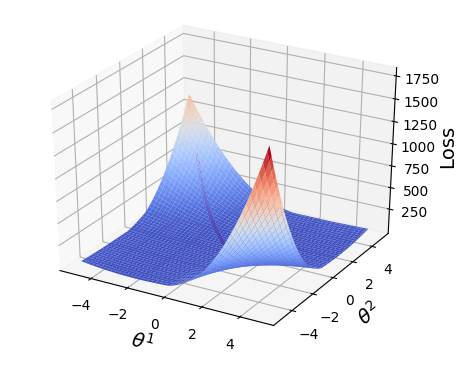
\includegraphics[width=\textwidth]{examples/1/3d.png}
		\caption{3D view on minimized function.}
		\label{fig:ex1:3d-view}
	\end{subfigure}
	\begin{subfigure}[b]{0.47\textwidth}
		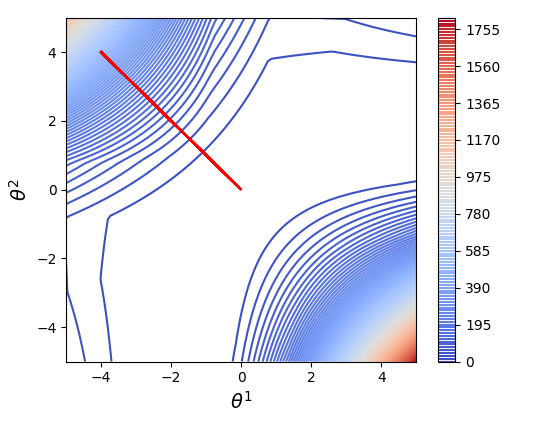
\includegraphics[width=\textwidth]{examples/1/2d.png}
		\caption{Hypsometric view on minimized function.}
		\label{fig:ex1:hypsometric}
	\end{subfigure}
	\caption{Plots of $MSE$ - Example 1.}
	\label{fig:ex1}
\end{figure}

Another example presented on Figure \ref{fig:ex2} shows same function, but this time algorithm start in point \texttt{[-4, -4]} and reaches minima at \texttt{[-2, -2.2]}.

\begin{figure}[!hbt]
\centering
	\begin{subfigure}[b]{0.47\textwidth}
		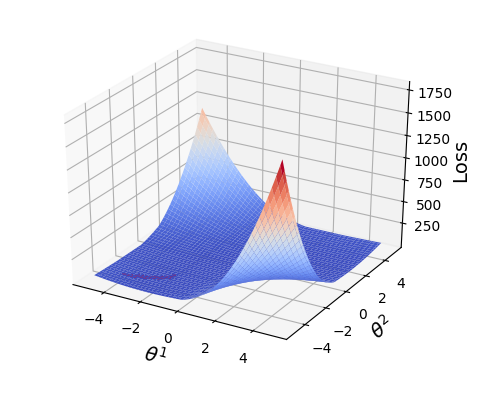
\includegraphics[width=\textwidth]{examples/2/3d.png}
		\caption{3D view on minimized function.}
		\label{fig:ex2:3d-view}
	\end{subfigure}
	\begin{subfigure}[b]{0.47\textwidth}
		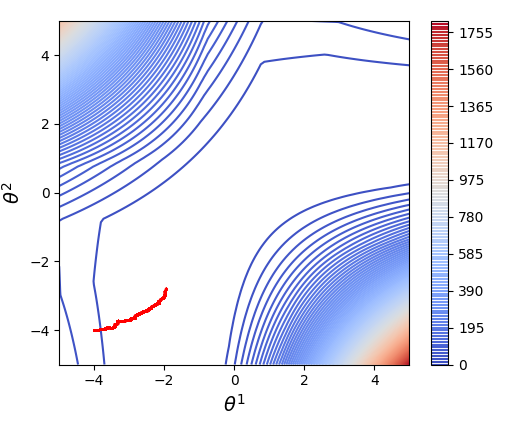
\includegraphics[width=\textwidth]{examples/2/2d.png}
		\caption{Hypsometric view on minimized function.}
		\label{fig:ex2:hypsometric}
	\end{subfigure}
	\caption{Plots of $MSE$ - Example 2.}
	\label{fig:ex2}
\end{figure}

Comparing both paths it can be observed that in first example algorithm was heading straight forward to minima, as it was falling from heap. Second example is starting in function plain, and steps are small, but very chaotic.

This examples are showing that algorithm is moving as fast as the function descent. Also, when descent is small, algorithm starts to move chaotic. The reason for this is that SGD is using subset of all observations, which comes with cost of loosing the precision.
\\

\subsubsection{Custom Function}

To also observe non standard function, authors have defined a Custom Error Function ($CEF$) and it is given by formula:
$$ CEF = \frac{1}{n}\sum_{t=1}^{n}sin^3(e_t) $$

This function does not have any real life appliance, but in case of this work, it can be used as an interesting abstract model.

In Figure \ref{fig:ex3} it can be observed the plot of such function. Very characteristic for periodic function $sin$ used in formula are many minimas (only two visible in this example) repeating in whole domain.

In this example algorithm start in point \texttt{[2, 0]} from which it moves to \texttt{[3, -2.2]} to one of minimas. When local minima is reached algorithm starts to float around local minima drifting forth and back to it.

\begin{figure}[!hbt]
\centering
	\begin{subfigure}[b]{0.47\textwidth}
		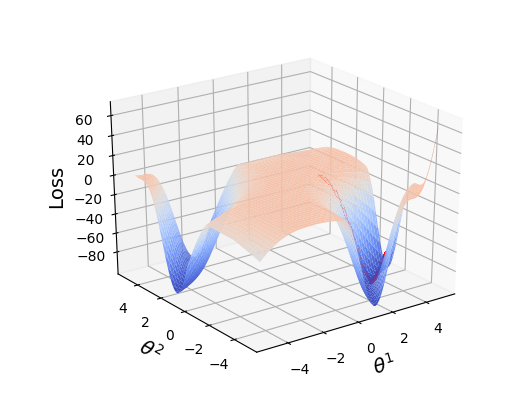
\includegraphics[width=\textwidth]{examples/3/3d.png}
		\caption{3D view on minimized function.}
		\label{fig:ex3:3d-view}
	\end{subfigure}
	\begin{subfigure}[b]{0.47\textwidth}
		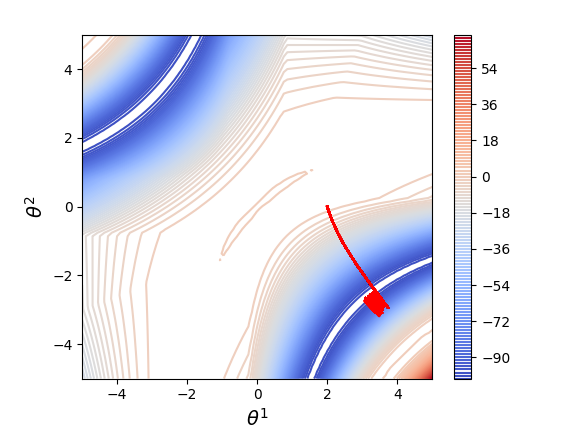
\includegraphics[width=\textwidth]{examples/3/2d.png}
		\caption{Hypsometric view on minimized function.}
		\label{fig:ex3:hypsometric}
	\end{subfigure}
	\caption{Plots of $CEF$ - Example 1.}
	\label{fig:ex3}
\end{figure}
	
The second example shown in Figure \ref{fig:ex4} show same function, but starting point is set to \texttt{[-2, 0]}. Algorithm has reached the other minima in \texttt{[-3.8, 3]}. The path thou, is the same - algorithm fastly reaches to minima and starts to drift around it in final steps.

\begin{figure}[!hbt]
\centering
	\begin{subfigure}[b]{0.47\textwidth}
		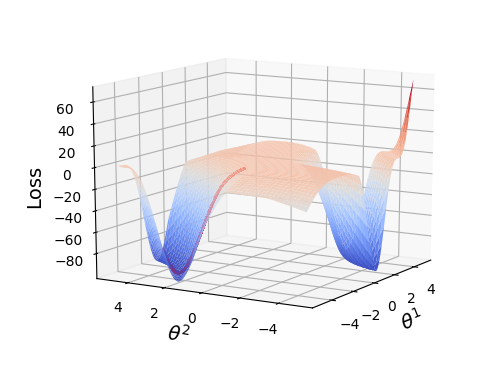
\includegraphics[width=\textwidth]{examples/4/3d.png}
		\caption{3D view on minimized function.}
		\label{fig:ex4:3d-view}
	\end{subfigure}
	\begin{subfigure}[b]{0.47\textwidth}
		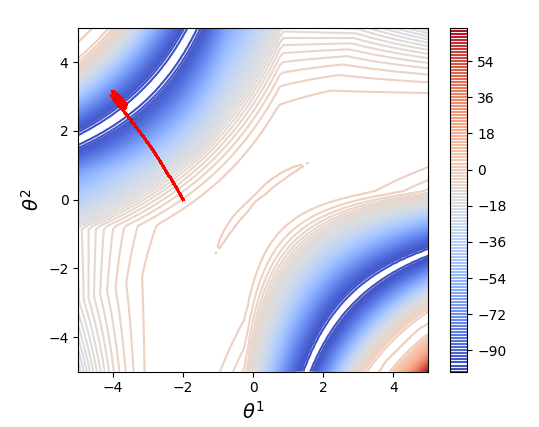
\includegraphics[width=\textwidth]{examples/4/2d.png}
		\caption{Hypsometric view on minimized function.}
		\label{fig:ex4:hypsometric}
	\end{subfigure}
	\caption{Plots of $CEF$ - Example 2.}
	\label{fig:ex4}
\end{figure}

This example is showing an impact of starting point to the algorithm - by selecting two different points, both runs have ended up with two different solutions for this optimilization. Of course, both results are correct and they should not be surprising, because, as it was mention before - goal function is periodic, so minimas will be repeating all over the domain. 

This function is also unique, because decent is not linear as it was in $MSE$ example. It causes slowing algorithm movement on lower descent, but with proper number of epoches minima is reached any way.

\subsection{Loss Value over epoches}

Another interesting aspect which can be observed using application is behaviour of Loss function over epoches. Plots in Figure \ref{fig:loss1} and Figure \ref{fig:loss2} are presenting results of $MSE$ and $CEF$ from previous examples accordingly.

In Figure \ref{fig:loss1:1} the descent starts at $800$ and it is very fast and very stable - each step is minimizing objective function. However, in Figure \ref{fig:loss1:2} the descent is chaotic, but the values are starting from lower level ($40$) than in first example.

\begin{figure}[!hbt]
	\begin{subfigure}[b]{0.45\textwidth}
		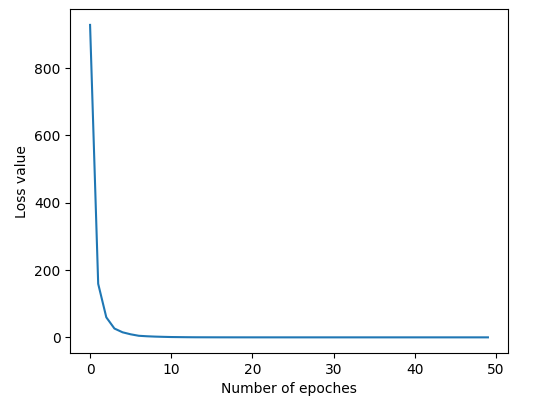
\includegraphics[width=\textwidth]{examples/1/loss.png}
		\caption{Example 1}
		\label{fig:loss1:1}
	\end{subfigure}
	\begin{subfigure}[b]{0.45\textwidth}
		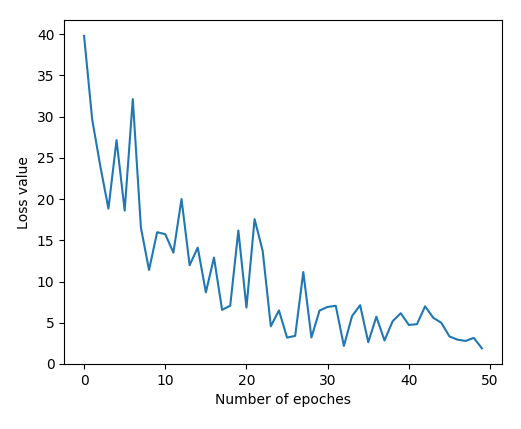
\includegraphics[width=\textwidth]{examples/2/loss.png}
		\caption{Example 2}
		\label{fig:loss1:2}
	\end{subfigure}
	\caption{Plot of loss value of $MSE$ over epoches}
	\label{fig:loss1}
\end{figure}

In Fugure \ref{fig:loss2:1} and \ref{fig:loss2:2} the shape of descent seems to be the same, but it is worth reminding that two different minimas were reached. As it was stated before descent is not linear, it starts slowly, and than accelerates very fast. Acot 10th epoch is reaches certain level and it drifts around it. 

\begin{figure}[!hbt]	
	\begin{subfigure}[b]{0.45\textwidth}
		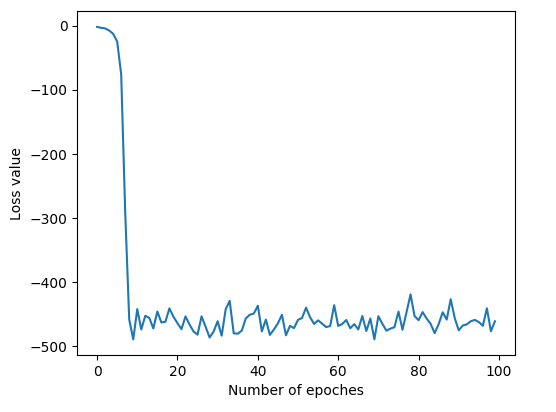
\includegraphics[width=\textwidth]{examples/3/loss.png}
		\caption{Example 1}
		\label{fig:loss2:1}
	\end{subfigure}
	\begin{subfigure}[b]{0.45\textwidth}
		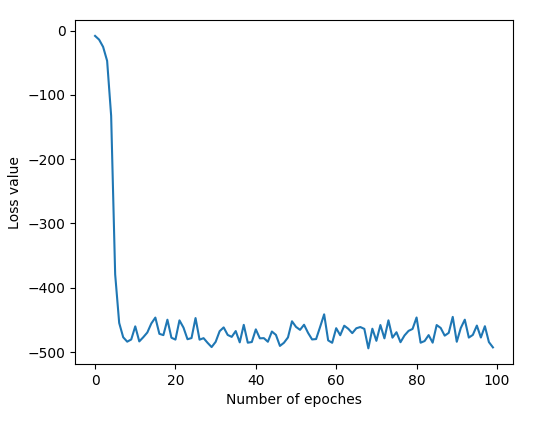
\includegraphics[width=\textwidth]{examples/4/loss.png}
		\caption{Example 2}
		\label{fig:loss2:2}
	\end{subfigure}
	\caption{Plot of $CEF$ loss value over epoches}
	\label{fig:loss2}
\end{figure}

In both cases, interpretation of plots is similar and it is reflecting tendencies of algorithm route. Such plots can be used to better analyse algorithm not only in cases covered by this work, but also more generic ones where number of variables is high and visualizing the path is impossible.

\section{Conclusion}
The Stochastic Gradient Algorithm gives a method for optimizing parameters of given function very fast. By taking advantage of probability, it allows to reduce a computational resources, especially on large datasets. In addition, animations rendered by application, can give an intuitive example to understand idea hidden by gradient descent methods.

\bibliography{sources}{}
\bibliographystyle{plain}

\end{document}